
\chapter{Objectifs.}

\chapter{Suivit de l'utilisateur.}
Dans le cahier des charges, l'utilisateur doit communiquer avec l'utilisateur grâce à un smartphone android. Nous décidons donc d'utiliser les ondes Wifi du smartphone pour trianguler sa position à l'aide de trois capteurs.

\paragraph{Remarque} Nous ne pouvons pas utiliser le GPS car il faudrait équiper notre robot d'un GPS et avoir une precision inférieure au mètre en intérieur, qui est le lieu de fonctionnement ciblé du project.

\section{Triangulation par durée de déplacement d'une onde.}
La première approche qui nous est venue est de mesurer le temps de trajet de l'onde électromagnétique du smartphone jusqu'aux capteurs. Si l'on place les capteurs de coordonnées connues $c_1(x_1;y_1;z_1)$, $c_2(x_2;y_2;z_2$ et $c_3(x_3;y_3;z_3)$. On cherche les coordonnées du smartphone $S(x;y;z)$ sachant les durées de trajet $t_1$, $t_2$ et $t_3$ de l'onde entre le smartphone et les capteurs. Comme une onde électromagnétique se déplace à la vitesse $c=299792458m.s^{-1}$, on peut déduire les distances qui séparent les capteurs du smartphone $d_1=t_1*c$, $d_2=t_2*c$ et $d_3=t_3*c$. On cherche donc à résoudre le système de trois équations à trois inconnues suivant (méthode de la \emph{trilatération}) :

\[
    \left|
    \begin{array}{rcl}
        (x-x_1)^2 + (y-y_1)^2 + (z-z_1)^2 &=& d_1^2 \\
        (x-x_2)^2 + (y-y_2)^2 + (z-z_2)^2 &=& d_2^2 \\
        (x-x_3)^2 + (y-y_3)^2 + (z-z_3)^2 &=& d_3^2 \\
    \end{array}
    \right.
\]

Cependant, comme nous sommes libres du placement de nos capteurs dans l'espace, on décide de la placer de le même plan $(x;y)$. De plus, on place les capteurs de façon à être sur les axe d'un repère orthonormé tel que $c_1(0;0;0)$, $c_2(d;0;0)$ et $c_3(0;d;0)$. $d$ étant une constante qui sera choisie lors de la construction. Les coordonnées du smartphone obtenues seront donc exprimées dans ce repère. Le système précédent est donc simplifié en :

\[
    \left|
    \begin{array}{rcl}
        x^2 + y^2 + z^2 &=& d_1^2 \\
        (x-d)^2 + y^2 + z^2 &=& d_2^2 \\
        x^2 + (y-d)^2 + z^2 &=& d_3^2 \\
    \end{array}
    \right.
\]

En soustrayant la première équation à la deuxième, on trouve :
\[
    \begin{array}{rcl}
        2xd &=& d_1^2-d_2^2 + d^2 \\
        x &=& \frac{d_1^2-d_2^2 + d^2}{2d} \\
    \end{array}
\]

\newpage
On a aussi $z^2 = d_1^2-x^2-y^2$ d'après la première équation. On le réinjecte dans la troisième équation :
\[ x^2+y^2-2yd+d^2+d_1^2-x^2-y^2 = d_3^2 \]
\[ y = -\frac{d_3^2-d_1^2-d^2}{2d} \]

On obtient donc :
\[
    S=\left|
    \begin{array}{rcl}
        x &=& \frac{d_1^2-d_2^2+d}{2d} \\
        y &=& -\frac{d_3^2-d_1^2-d^2}{2d} \\
        z &=& \pm\sqrt{d_1^2-x^2-y^2} \\
    \end{array}
    \right.
\]

On constate qu'il peut y avoir 0, 1 ou 2 solution pour $z$ dans $\mathbb{R}$. Ceci n'est pas vraiment important car notre robot se déplace uniquement dans un plan, et la valeur de $z$ n'influe pas sur sa trajectoire. Cette valeur n'est utile que lorsque nous voulons connaitre la distance entre le robot et le smartphone.

Afin de tester la véracité de ces formules, nous codons un test basé sur plusieurs programmes. Le premier programme est celui qui va être utilisé dans le PPE : il reçoit les temps entre le smartphone et les capteurs et retourne la position du capteur. Le deuxième programme utilisé reçoit les coordonnées du smartphone, calcule les temps de trajet, les transmet au premier programme et compare les coordonnées obtenues avec celles de départ. En se basant uniquement sur cette suite de test, il apparait que nos équations sont bonnes : on retrouve bien les coordonnées du smartphone avec une précision au millième de millimètre.

Cependant, afin de dimensionner nos circuits, on utilise un troisième script qui va générer des coordonnées aléatoirement, va les passer au second programme qui va arrondir les temps à une precision données et va retourner une erreur si l'écart entre les coordonnées est trop grand. Nous fixons ce \emph{trop grand} à \emph{> 50cm}, car une précision à \emph{50cm} est suffisante pour le suivit de la personne. Il en ressort que pour avoir une précision dans les coordonnées de cet ordre là, il faut une précision dans la mesure du temps à $10^{-11}s$. Cette précision n'est bien sûr pas atteignable avec nos moyen.

Nous devons donc trouver une nouvelle approche pour obtenir les coordonnées du smartphone.

\section{Triangulation par mesure d'intensité.}
La seconde approche s'inspire des petits robot suiveurs de lumière que l'on peut trouver un peut partout sur le net. L'idée est de mesurer l'intensité du signal qui arrive à chacun des capteurs et d'en déduire les coordonnées du smartphone. En effet, un flux d'ondes électromagnétiques suit la loi du carré inverse, c'est à dire que son intensité décroit avec le carré de la distance parcourue. Cette approche possède deux avantages principaux : \begin{enumerate}
    \item Il n'est pas nécessaire d'avoir des informations sur le smartphone : l'intégralité du traitement peut se faire sur le robot, ce qui simplifie la mise en œuvre.
    \item Si nous n'arrivons pas à trouver les formules mathématiques pour déduire les coordonnées du smartphone, nous pourrons toujours le suivre en comparant l'intensité du flux d'onde qui arrive aux capteurs.
\end{enumerate}

Nous allons centrer notre étude sur deux capteurs, afin de voir ce que nous pouvons obtenir. Nous nommons les capteurs $c_1$ et $c_2$. Nous avons les distance $d_1$ et $d_2$ entre le smartphone et ces capteurs ainsi que $I$ l'intensité initiale du flux, que nous ne connaissons pas. Les intensités que nous mesurons sur les capteurs sont $I_1=I*d_1^{-2}$ et $I_2=I*d_2^{-2}$. Afin de supprimer les $I$ (valeur inconnue), nous allons nous intéresser au rapport :
\[ \frac{I_1}{I_2} = \frac{d_2^2}{d_1^2} \Leftrightarrow k=\sqrt{\frac{I_1}{I_2}}=\frac{d_2}{d_1} \]

Afin de déterminer quel genre d'équation nous allons obtenir, nous utilisons un programme qui dessine une forme géométrique telle que $\frac{d_1}{d_2} = cte$. Après différents tests(voir figure \ref{follow_conj}), nous conjecturons qu'il s'agit d'un cercle.

\begin{figure}
    \label{follow_conf}
    \begin{center}
        \begin{tabular}{cc}
            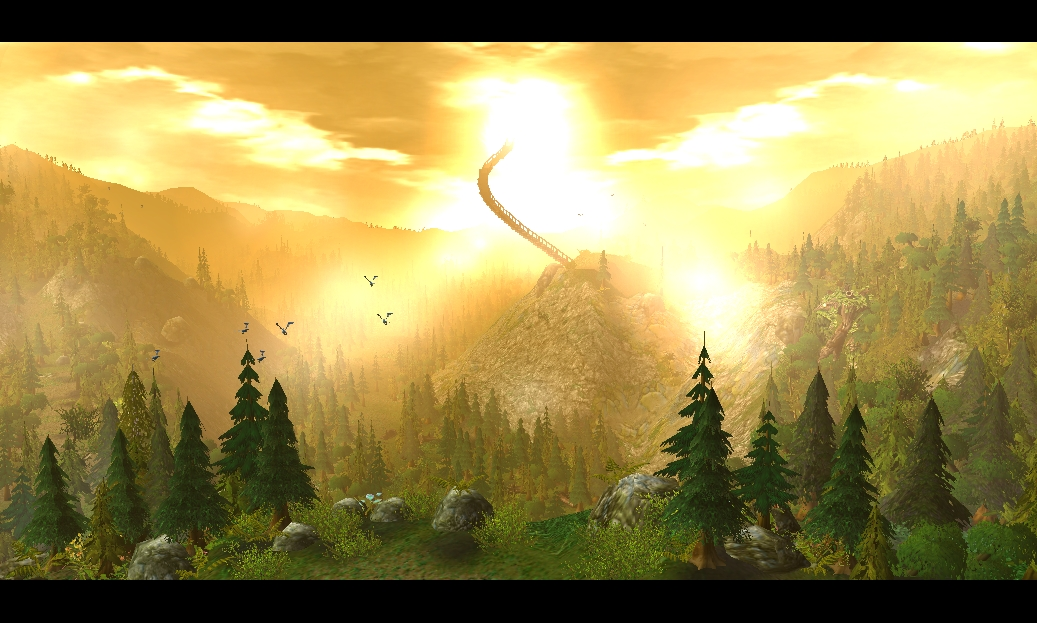
\includegraphics[width=0.4\linewidth]{rcs/follow1.png} & 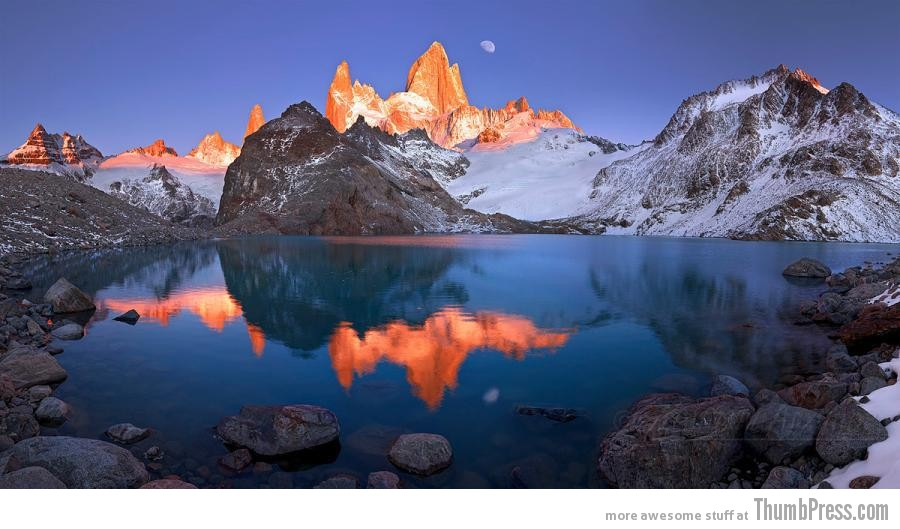
\includegraphics[width=0.4\linewidth]{rcs/follow2.png}
        \end{tabular}
    \end{center}
    \caption{Figures géométriques définies par un rapport de distance.}
\end{figure}

Cependant, il ne nous a pas été possible de trouver de capteur permettant la mesure de l'intensité d'une onde électromagnétique : nous avons donc du abandonner cette approche, au delà de la difficulté mathématique de gérer cette approche. Ceci amène la troisième approche.

\section{Suivit par caméra.}
\subsection{Présentation.}
Cette approche vient de l'incapacité de mener à bout les deux précédentes approches et de la présence d'une unité capable de gérer des flux vidéo en temps réel pour la détection d'obstacle.

Cette approche possède de très nombreuses limites, qui l'empêche d'être une solution définitive. Nous la considérons quand même suffisante pour nos besoin, et entre dans nos capacités. Parmi ces limites, on peut citer le fait qu'il faut que l'utilisateur soit toujours dans le champ de vision de la caméra. De plus, le reconnaissance se basant sur la couleur, il faut que l'utilisateur porte un vêtement de cette couleur. Enfin, si un objet ou une personne ayant la même couleur que celle suivit entre dans le champ de vision du robot, cela risque de le perturber, et il risque de se mettre à suivre autre chose que l'utilisateur.

\subsection{Fonctionnement.}
Il n'y a pas de concept mathématique derrière cette approche : le robot va juste capter une image et effectuer une série de transformations dessus pour en tirer les coordonnées de l'utilisateur sur l'image, puis il verra où se il se situe par rapport à lui pour décider de la direction à prendre.

Les différentes étapes de la transformation sont : \begin{enumerate}
    \item L'image obtenue est mise dans l'espace de couleur \emph{HSV} (\emph{Hue}, \emph{Saturation}, \emph{Value}, soit teinte, saturation, valeur en français) : cet espace de couleur d'identifier une couleur en séparant cette information de l'intensité lumineuse et de la saturation, ce qui permet de retrouver la couleur même si elle est altérée par la luminosité ambiante. % TODO figure pour HSV
    \item L'image est ensuite binarisée suivant un modèle très simple : les trois composantes sont testées, vérifiant si elles font parties d'un encadrement préalablement déterminé. Si les trois sont validé, le pixel est mis à 1 (couleur blanche), sinon il est mis à 0 (couleur noir). Afin de déterminer ces encadrements, un programme de test a été écrit permettant de les modifier dynamiquement pour voir la meilleur combinaison possible. % TODO screenshot du programme
    \item Un algorithme de détection de contours est ensuite appliqué à l'image pour obtenir la liste des tâche blanches sur l'image. Leur aire est calculée et seule la tâche blanche avec l'aire la plus importante est gardée, ce qui permet d'éliminer les faux positifs. Si l'aire de la tâche la plus grande est trop petite, le programme considère que l'utilisateur est sorti de son champ de vision et se stoppe.
    \item Le rectangle encadrant le contour maximum est calculé, puis son centre en est déduit. Le point ainsi obtenu est considéré comme étant la position de l'utilisateur dans l'image.
        %TODO Figure présentant les différentes étapes
\end{enumerate}

\chapter{Détection des obstacles.}

\chapter{Contrôle.}

